\section{Inverse Problem}

While the forward heat diffusion problem consists of predicting the temperature evolution from known physical parameters, the inverse problem is fundamentally more challenging. In the inverse formulation, the objective is no longer only to compute the solution of the governing equation itself, but rather to infer unknown physical quantities directly from partial and potentially noisy observations. In this work, the inverse problem focuses on estimating the thermal diffusivity coefficient $\alpha$ from sparse temperature measurements distributed in space and time. Inverse problems are particularly important in science and engineering because many real-world situations involve unknown physical parameters that cannot be measured directly. Instead, these quantities must be reconstructed indirectly from experimental observations.

Examples include:
\begin{itemize}
    \item thermal property identification, e.g., estimating the thermal
    diffusivity or conductivity of a material from temperature measurements;

    \item material characterization, e.g., identifying elastic moduli,
    permeability, or constitutive-law parameters from experimental data;

    \item medical imaging, e.g., reconstructing tissue properties or internal
    structures from MRI, ultrasound, or computed tomography measurements;

    \item fluid dynamics parameter estimation, e.g., estimating viscosity,
    boundary conditions, or unknown source terms from velocity and pressure data;

    \item geophysical inversion, e.g., reconstructing subsurface properties
    such as seismic-wave velocity or permeability from surface measurements;

    \item multiphysics system calibration, e.g., estimating coupled thermal,
    mechanical, or electromagnetic parameters from observations of the system.
\end{itemize}

Traditional numerical approaches for inverse problems often rely on repeated calls to classical PDE solvers inside iterative optimization loops. While these methods can be highly accurate, they may become computationally expensive when the parameter space is large, the governing equations are nonlinear, the geometry is complex, or experimental data are sparse and noisy. Physics-Informed Neural Networks (PINNs) provide an alternative framework where the physical solution and the unknown parameters can be learned simultaneously within a single optimization process. This constitutes one of the main motivations behind PINNs and scientific machine learning approaches.

% =========================================================
\subsection{Why PINNs Are Particularly Interesting for Inverse Problems}
% =========================================================

Unlike standard forward simulations, inverse problems represent a domain where PINNs may offer significant advantages compared to traditional numerical solvers. The neural network approximates the solution field, while unknown physical parameters are optimized simultaneously during training. For the present 1D thermal diffusion problem, the thermal diffusivity coefficient $\alpha$ becomes a trainable parameter of the optimization process. The inverse PINN therefore attempts to minimize both discrepancies with observational data, and violations of the governing PDE.

This allows PINNs to naturally integrate:
\begin{itemize}
    \item sparse observations, e.g., temperature measurements available at only
    a limited number of spatial and temporal locations;

    \item noisy experimental measurements, e.g., temperature data affected by
    sensor noise or measurement uncertainty;

    \item physical constraints, e.g., governing equations, initial conditions,
    boundary conditions, or conservation laws;

    \item parameter estimation, e.g., identifying an unknown thermal diffusivity
    $\alpha$ from sparse and noisy temperature measurements.
\end{itemize}

within a unified differentiable framework. In contrast with many traditional inverse approaches, PINNs do not necessarily require repeated external PDE solves during optimization, since the PDE residual is directly embedded inside the loss function through automatic differentiation. However, although PINNs are conceptually attractive for inverse problems, they also introduce important optimization and identifiability challenges.

% =========================================================
\subsection{Inverse Problem Formulation}
% =========================================================

The inverse problem considered in this work consists of estimating the
thermal diffusivity $\alpha$ from noisy temperature observations. Since no
physical experiments were conducted, synthetic temperature measurements
were generated using the following analytical solution:

\begin{equation}
T_{\mathrm{exact}}(x,t)
=
\sin\left(\frac{\pi x}{L}\right)
\exp\left[
-\alpha
\left(\frac{\pi}{L}\right)^2 t
\right].
\end{equation}

To simulate experimental measurement uncertainty, additive Gaussian noise
was introduced:

\begin{equation}
T_{\mathrm{obs},i}
=
T_{\mathrm{exact}}(x_i,t_i)
+
\varepsilon_i,
\end{equation}

where

\begin{equation}
\varepsilon_i \sim \mathcal{N}(0,\sigma^2),
\end{equation}

and $\sigma$ denotes the standard deviation of the measurement noise. As mentionned earlier, the PINN must therefore simultaneously:
\begin{itemize}
    \item reconstruct the temperature field,
    \item satisfy the governing PDE,
    \item and infer the correct value of $\alpha$.
\end{itemize}

\begin{figure}
    \centering
    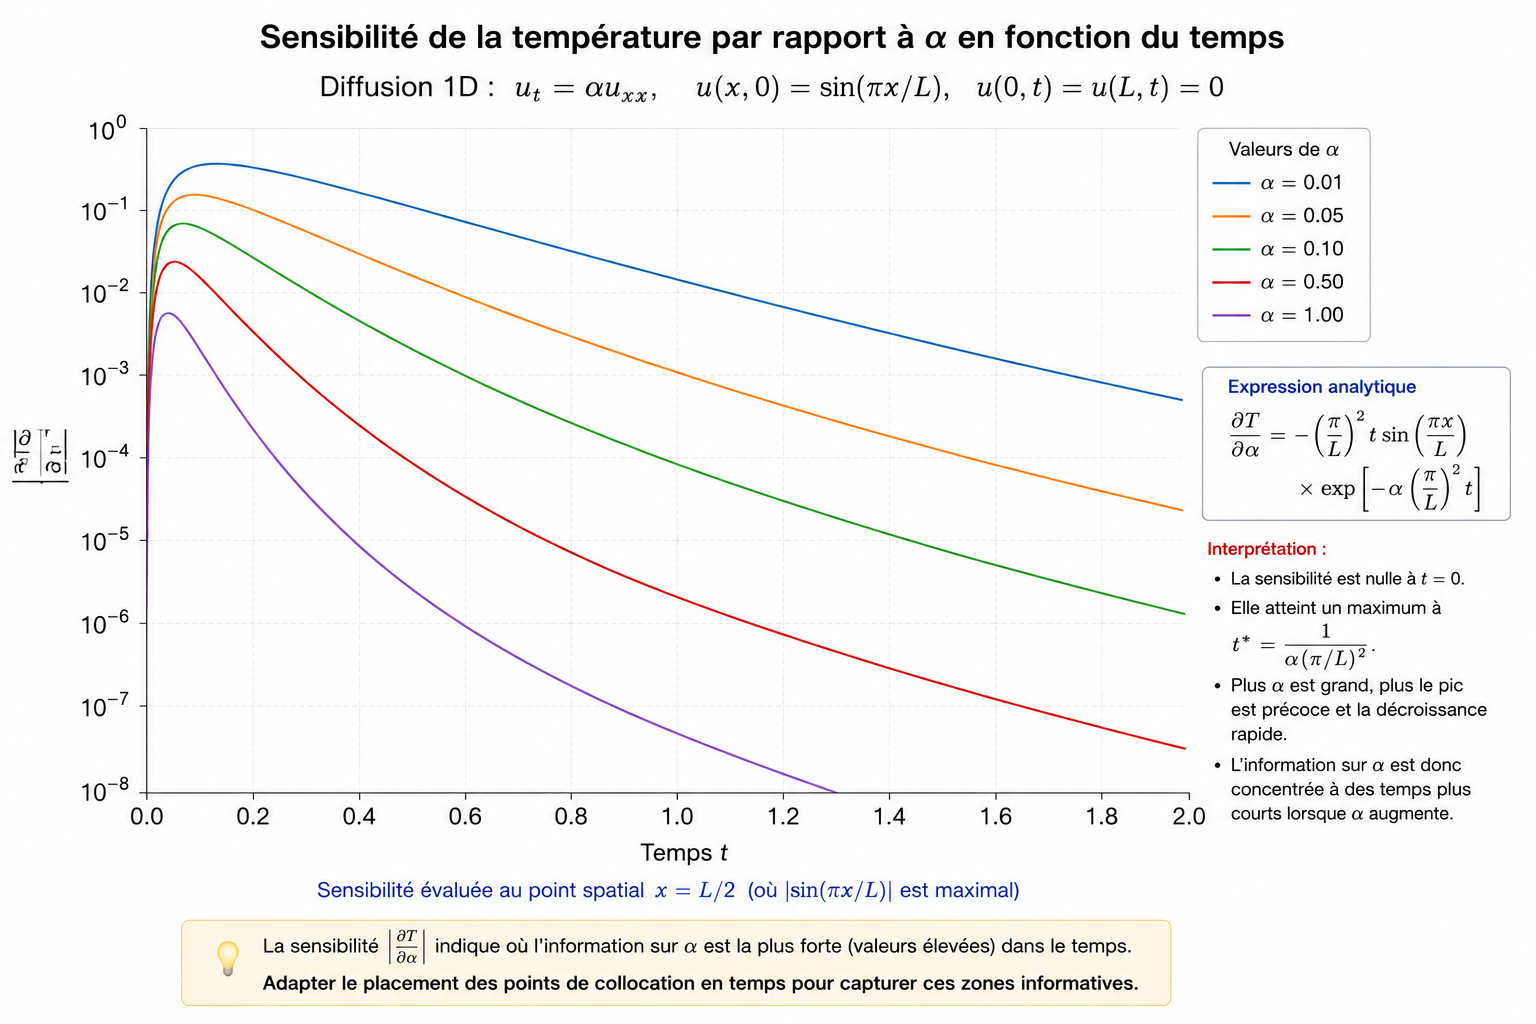
\includegraphics[width=0.75\linewidth]{figures/derive_alpha.png}
    \caption{Informative choice of alpha}
    \label{fig:derive_alpha}
\end{figure}

% =========================================================
\subsection{Soft and Hard Constraint Strategies}
% =========================================================

\subsection{Enforcement of Initial and Boundary Conditions}

An important aspect investigated in this work is the enforcement of the
initial and boundary conditions. Two strategies were explored: soft and hard
constraint enforcement.

\paragraph{Soft constraints}

In the soft-constrained formulation, the initial and boundary conditions are
enforced by adding penalty terms to the total loss function:

\begin{equation}
\mathcal{L}_{\mathrm{total}}
=
\lambda_{\mathrm{physics}}\mathcal{L}_{\mathrm{physics}}
+
\lambda_{\mathrm{data}}\mathcal{L}_{\mathrm{data}}
+
\lambda_{\mathrm{initial}}\mathcal{L}_{\mathrm{initial}}
+
\lambda_{\mathrm{boundary}}\mathcal{L}_{\mathrm{boundary}}.
\end{equation}

This approach is straightforward and flexible because it does not require the
construction of a particular analytical form for the network output. It can
therefore be applied relatively easily to different initial and boundary
conditions, including problems involving complex geometries. Soft constraints
are also useful when the prescribed conditions are uncertain or affected by
measurement noise, since potentially inaccurate values are not imposed exactly.
Moreover, the relative importance of each condition can be adjusted through its
weighting coefficient. However, this flexibility introduces several limitations:

\begin{itemize}
   \item the initial and boundary conditions are generally satisfied only
    approximately;
    \item the different components of the loss function must be appropriately
    balanced and therefore the training results may be sensitive to the weighting coefficients
    $\lambda_{\mathrm{initial}}$ and $\lambda_{\mathrm{boundary}}$;
    \item competing loss terms may lead to optimization difficulties and slower
    convergence.
\end{itemize}

\paragraph{Hard constraints}

In the hard-constrained formulation, the predicted solution is analytically
constructed so that the initial and boundary conditions are satisfied exactly
for any values of the neural-network parameters. For the one-dimensional heat
equation considered in this work, the constrained solution is written as

\begin{equation}
T_{\theta}(x,t)
=
\sin\left(\frac{\pi x}{L}\right)
+
t\,x(L-x)\,N_{\theta}(x,t),
\end{equation}

where $N_{\theta}(x,t)$ is the unconstrained output of the neural network. At
$t=0$, the second term vanishes, and the prescribed initial condition $T_{\theta}(x,0) = \sin\left(\frac{\pi x}{L}\right)$ is
recovered. Similarly, the factor $x(L-x)$ vanishes at $x=0$ and $x=L$, ensuring
that the homogeneous $T_{\theta}(0,t) = T_{\theta}(L,t) = 0$ boundary conditions are satisfied. This formulation offers several advantages:

\begin{itemize}
    \item the initial and boundary conditions are satisfied exactly by design;
    \item the corresponding penalty terms and weighting coefficients are removed
    from the loss function and so the optimization problem contains fewer competing objectives;
    \item physical consistency, optimization stability, and convergence robustness
    can be improved.
\end{itemize}

Nevertheless, hard constraints also have limitations:

\begin{itemize}
    \item an appropriate constrained analytical form must be derived for the
    specific problem;
    \item this construction may become difficult for complex geometries, mixed or
    time-dependent boundary conditions, and multiphysics problems;
    \item inaccurate or noisy prescribed conditions are imposed exactly, which may
    introduce bias into the predicted solution;
    \item the chosen transformation can affect the scaling and optimization of the
    neural-network correction.
\end{itemize}

In the present problem, the geometry and prescribed conditions are sufficiently
simple to construct an explicit hard-constrained solution. This strategy was
therefore progressively adopted to reduce the number of loss terms and improve
the robustness of the inverse identification procedure. However, soft
constraints remain more flexible and may be preferable when the conditions are
uncertain or when an exact constrained formulation is difficult to derive.

% =========================================================
\subsection{Low-Amplitude Solutions and Parameter Identifiability}
% =========================================================

One of the main challenges encountered in the inverse PINN framework was the
loss of identifiability of the thermal diffusivity $\alpha$ when the predicted
temperature field becomes small. For the one-dimensional heat equation,

\begin{equation}
\frac{\partial T}{\partial t}
=
\alpha
\frac{\partial^2 T}{\partial x^2},
\end{equation}

the physics residual is defined as

\begin{equation}
R_\theta(x,t;\alpha)
=
\frac{\partial T_\theta}{\partial t}
-
\alpha
\frac{\partial^2 T_\theta}{\partial x^2}.
\end{equation}

The identically zero field,

\begin{equation}
T_\theta(x,t)=0,
\end{equation}

is a solution of the homogeneous heat equation for any value of $\alpha$.
Consequently, if the initial and boundary conditions are not sufficiently
enforced and the observational data do not prevent it, the network may approach
a low-amplitude solution that produces a small physics loss without correctly
identifying $\alpha$.

It should be emphasized that a small temperature amplitude does not, in
general, imply small temporal or spatial derivatives. A low-amplitude function
may still exhibit large derivatives, particularly if it contains rapid
variations. However, for the analytical solution considered in this work,

\begin{equation}
T_{\mathrm{exact}}(x,t)
=
\sin\left(\frac{\pi x}{L}\right)
\exp\left[
-\alpha
\left(\frac{\pi}{L}\right)^2 t
\right],
\end{equation}

both relevant derivatives are directly proportional to the temperature field:

\begin{equation}
\frac{\partial T_{\mathrm{exact}}}{\partial t}
=
-\alpha
\left(\frac{\pi}{L}\right)^2
T_{\mathrm{exact}},
\end{equation}

and

\begin{equation}
\frac{\partial^2 T_{\mathrm{exact}}}{\partial x^2}
=
-
\left(\frac{\pi}{L}\right)^2
T_{\mathrm{exact}}.
\end{equation}

Therefore, as the solution decays, its temporal derivative and spatial
curvature also decrease. This progressively reduces the information available
for estimating $\alpha$.

Indeed, the sensitivity of the residual to the unknown parameter is

\begin{equation}
\frac{\partial R_\theta}{\partial \alpha}
=
-
\frac{\partial^2 T_\theta}{\partial x^2}.
\end{equation}

When the spatial curvature becomes small, changes in $\alpha$ have little
influence on the residual. The physics loss may then remain small over a broad
range of $\alpha$ values, leading to a poorly conditioned parameter
identification problem.

This difficulty becomes particularly important for large values of the true
diffusivity. In this regime, the temperature field decays rapidly and
late-time observations contain little information about $\alpha$. As a
consequence:

\begin{itemize}
    \item the signal amplitude and spatial curvature decrease rapidly;
     \item the loss becomes less sensitive to the value of $\alpha$;
    \item the signal-to-noise ratio deteriorates and different values of $\alpha$ may produce temperature predictions
    that are difficult to distinguish within the measurement noise.
\end{itemize}

This behavior highlights an important distinction between solution
reconstruction and parameter identification. A PINN may reconstruct a
low-amplitude temperature field with a small prediction error while still
providing an inaccurate estimate of $\alpha$. Accurate parameter recovery
therefore requires observations in regions of the space--time domain where the
solution remains sufficiently sensitive to the unknown diffusivity.

% =========================================================
\subsubsection{Parameter Reparameterization}
% =========================================================

The thermal diffusivity must satisfy

\begin{equation}
\alpha > 0,
\end{equation}

because heat flows from hotter to colder regions. A negative diffusivity would
instead describe an unphysical anti-diffusion process. Directly optimizing $\alpha$ does not guarantee that this physical constraint
will be respected during training. Gradient-based updates may lead to negative
or unrealistically small values, particularly during the early stages of
optimization, when the temperature field has not yet been accurately
reconstructed. To enforce a positive lower bound, a new trainable variable $\beta$ is
introduced such that

\begin{equation}
\alpha
=
\alpha_{\mathrm{floor}}
+
\beta^2,
\end{equation}

where $\alpha_{\mathrm{floor}}>0$ is a prescribed minimum admissible value.
The optimizer updates $\beta$, while $\alpha$ is reconstructed from this
expression during each evaluation of the loss function. This guarantees that

\begin{equation}
\alpha
\geq
\alpha_{\mathrm{floor}}
>
0.
\end{equation}

The effect of this transformation on the optimization dynamics can be understood
using the chain rule:

\begin{equation}
\frac{\partial \mathcal{L}}{\partial \beta}
=
\frac{\partial \mathcal{L}}{\partial \alpha}
\frac{d\alpha}{d\beta}
=
2\beta
\frac{\partial \mathcal{L}}{\partial \alpha}.
\end{equation}

As $\alpha$ approaches $\alpha_{\mathrm{floor}}$, $\lvert\beta\rvert$ becomes
small and the gradient transmitted to $\beta$ is progressively reduced. The
evolution of the physical parameter therefore slows down near its lower bound.
This can prevent $\alpha$ from decreasing too rapidly during the early stages
of training and give the neural network more time to reconstruct the
temperature field. However, the square transformation also has limitations. If $\beta$ becomes
very close to zero, the gradient with respect to $\beta$ may become extremely
small, making it difficult for $\alpha$ to move away from its lower bound.
Moreover, the mapping is not one-to-one, since $\beta$ and $-\beta$ correspond
to the same value of $\alpha$. The reparameterization guarantees physical
admissibility and modifies the parameter-learning dynamics, but it does not
guarantee that the correct value of $\alpha$ will be identified. Other approaches may also be used to constrain the unknown parameter:

\begin{itemize}
    \item \textbf{Softplus reparameterization:}
    \begin{equation}
    \alpha
    =
    \alpha_{\mathrm{floor}}
    +
    \operatorname{softplus}(\beta),
    \end{equation}
    which provides a smooth positive mapping and avoids the zero derivative of
    the square transformation at $\beta=0$;

    \item \textbf{Exponential reparameterization:}
    \begin{equation}
    \alpha
    =
    \alpha_{\mathrm{floor}}
    +
    \exp(\beta),
    \end{equation}
    which guarantees positivity but can generate very large parameter values
    and gradients;

    \item \textbf{Bounded sigmoid reparameterization:}
    \begin{equation}
    \alpha
    =
    \alpha_{\min}
    +
    \left(\alpha_{\max}-\alpha_{\min}\right)
    \operatorname{sigmoid}(\beta),
    \end{equation}
    which is appropriate when physically justified lower and upper bounds are
    known, although gradient saturation may occur near these bounds;

    \item \textbf{Bound-constrained optimization:} the parameter is directly
    restricted to an admissible interval using projection or a constrained
    optimization algorithm;

    \item \textbf{Penalty-based regularization:} an additional term is introduced
    into the loss function to penalize negative or physically implausible values
    of $\alpha$.
\end{itemize}

In the present work, the square reparameterization was selected because it is
simple to implement, guarantees a positive diffusivity, and reduces rapid
variations of $\alpha$ near the prescribed lower bound. Nevertheless, its
effectiveness still depends on the initialization of $\beta$, the balance
between the data and physics losses, and the sensitivity of the observations
to $\alpha$.

% =========================================================
\subsubsection{Sensitivity-Based Weighting}
% =========================================================

Even after introducing observational data and parameter reparameterization,
inverse parameter identification remains challenging because the measurements do
not all contain the same amount of information about the unknown diffusion
coefficient $\alpha$. Sensitivity-based weighting was therefore investigated to
increase the influence of the observations that are the most informative for
parameter identification.

For the analytical solution considered in this work,

\begin{equation}
T_{\mathrm{exact}}(x,t)
=
\sin\left(\frac{\pi x}{L}\right)
\exp\left[
-\alpha
\left(\frac{\pi}{L}\right)^2 t
\right],
\end{equation}

the sensitivity of the temperature to the diffusion coefficient is

\begin{equation}
S_{\alpha}(x,t)
=
\frac{\partial T_{\mathrm{exact}}}{\partial \alpha}
=
-
\left(\frac{\pi}{L}\right)^2
t
\sin\left(\frac{\pi x}{L}\right)
\exp\left[
-\alpha
\left(\frac{\pi}{L}\right)^2 t
\right].
\end{equation}

The magnitude

\begin{equation}
\left|S_{\alpha}(x,t)\right|
=
\left|
\frac{\partial T_{\mathrm{exact}}}{\partial\alpha}
\right|
\end{equation}

measures the local variation of the temperature caused by a small change in
$\alpha$. A large value indicates that the observation is strongly affected by
the diffusion coefficient and therefore contains useful information for its
identification. Conversely, a small value indicates that substantially different
values of $\alpha$ may produce similar temperature values at that location.

% =========================================================
\paragraph{Weighted data loss}
% =========================================================

The sensitivity weights are applied to the individual temperature-error terms in
the data loss. For a set of $N_d$ observations, the weighted data loss is defined
as

\begin{equation}
\mathcal{L}_{\mathrm{data}}^{(w)}
=
\frac{
\displaystyle
\sum_{i=1}^{N_d}
w_i
\left[
T_{\theta}(x_i,t_i)-T_{\mathrm{obs},i}
\right]^2
}{
\displaystyle
\sum_{i=1}^{N_d} w_i
}.
\end{equation}

Normalization by the sum of the weights keeps the scale of the data loss
approximately independent of the selected weighting law and of the overall
magnitude of the sensitivities. The weights therefore redistribute the relative
contributions of the observations without arbitrarily changing the global scale
of the data-fitting term.

Several sensitivity-based weighting laws were examined:

\begin{align}
w_i
&=
\left|S_{\alpha}(x_i,t_i)\right|,
\\
w_i
&=
S_{\alpha}(x_i,t_i)^2,
\\
w_i
&=
\sqrt{
\left|S_{\alpha}(x_i,t_i)\right|
}.
\end{align}

Quadratic weighting strongly concentrates the data loss on the observations with
the largest sensitivities. This may reduce the effective use of the remaining
dataset and make the optimization more sensitive to a limited number of points.
Linear weighting produces a less concentrated distribution, but may still create
a strong contrast between informative and weakly informative measurements.

In the experiments conducted here, the square-root formulation provided a useful
compromise. It increased the contribution of informative observations while
maintaining a broader participation of the available dataset.

% =========================================================
\paragraph{Why sensitivity weights are applied only to the data loss}
% =========================================================

The sensitivity weights are applied only to the data loss because they quantify
the information carried by each temperature observation about the unknown
parameter $\alpha$. Their purpose is to redistribute the contribution of the
measured data according to their relevance for parameter identification.

The other loss terms have fundamentally different roles. The physics loss is
defined as

\begin{equation}
\mathcal{L}_{\mathrm{physics}}
=
\frac{1}{N_f}
\sum_{j=1}^{N_f}
\left[
\frac{\partial T_{\theta}}{\partial t}(x_j^f,t_j^f)
-
\alpha
\frac{\partial^2T_{\theta}}{\partial x^2}(x_j^f,t_j^f)
\right]^2,
\end{equation}

where $(x_j^f,t_j^f)$ are the collocation points. This term enforces the heat
equation throughout the space--time domain. Its objective is not to quantify the
information content of an observation, but to ensure that the predicted
temperature field is physically admissible.

Applying the same sensitivity weights to the physics residual would weaken the
enforcement of the governing equation in regions where
$|\partial T/\partial\alpha|$ is small. The PINN could consequently tolerate
larger physics errors near the boundaries, at early times, or at late times, even
though the heat equation remains valid and must be satisfied in all of these
regions.

The same reasoning applies to possible initial- and boundary-condition losses.
These terms impose the constraints that define the forward problem rather than
measurements whose purpose is to identify $\alpha$. In the present problem,

\begin{equation}
S_{\alpha}(x,0)=0,
\qquad
S_{\alpha}(0,t)=S_{\alpha}(L,t)=0.
\end{equation}

Consequently, applying sensitivity weights to the initial-condition loss would
assign zero importance to the prescribed initial temperature profile. Similarly,
applying them to the boundary-condition loss would suppress the constraints at
$x=0$ and $x=L$. This could allow violations of the initial or boundary
conditions precisely where they must be enforced.

The distinction can therefore be summarized as follows: sensitivity weighting
determines which observations should influence parameter identification most
strongly, whereas the physics, initial-condition, and boundary-condition terms
define the set of physically admissible solutions. The total loss may thus be
written as

\begin{equation}
\mathcal{L}_{\mathrm{total}}
=
\lambda_{\mathrm{data}}
\mathcal{L}_{\mathrm{data}}^{(w)}
+
\lambda_{\mathrm{physics}}
\mathcal{L}_{\mathrm{physics}}
+
\lambda_{\mathrm{IC}}
\mathcal{L}_{\mathrm{IC}}
+
\lambda_{\mathrm{BC}}
\mathcal{L}_{\mathrm{BC}},
\end{equation}

with the sensitivity weights applied only inside
$\mathcal{L}_{\mathrm{data}}^{(w)}$. When the initial and boundary conditions are
imposed through a hard-constraint transformation, as in part of the present
study, the corresponding losses are absent and the total loss reduces to

\begin{equation}
\mathcal{L}_{\mathrm{total}}
=
\lambda_{\mathrm{data}}
\mathcal{L}_{\mathrm{data}}^{(w)}
+
\lambda_{\mathrm{physics}}
\mathcal{L}_{\mathrm{physics}}.
\end{equation}

This choice does not imply that the other loss terms can never be weighted.
Adaptive residual weighting or nonuniform collocation sampling may, for example,
be used to improve the enforcement of the governing equation in difficult
regions. Such physics-oriented strategies pursue a different objective and
should be based on the residual, its derivatives, or an appropriate error
indicator rather than automatically reusing weights designed to measure the
parameter information contained in observations.

% =========================================================
\paragraph{Physical interpretation of the sensitivity distribution}
% =========================================================

For the present problem, the spatial and temporal distributions of sensitivity
can be understood directly from the underlying physics. At the initial time,

\begin{equation}
S_{\alpha}(x,0)=0,
\end{equation}

because the prescribed initial temperature profile is independent of $\alpha$.
The diffusion coefficient controls the subsequent evolution of the field, but not
its initial value. Consequently, measurements taken exactly at $t=0$ contain no
direct information about $\alpha$.

At very early times, diffusion has only weakly modified the initial temperature
profile, so the effect of $\alpha$ remains limited. At late times, the temperature
field has largely decayed and may become comparable to the measurement noise.
Both the signal amplitude and its sensitivity to $\alpha$ then become small.
Intermediate times are therefore generally the most informative: diffusion has
acted sufficiently for the influence of $\alpha$ to become observable, while the
temperature signal has not yet disappeared.

For a fixed spatial location, the sensitivity magnitude is proportional to

\begin{equation}
t
\exp\left[
-\alpha
\left(\frac{\pi}{L}\right)^2t
\right].
\end{equation}

Differentiating this expression with respect to time shows that it reaches its
maximum at

\begin{equation}
t_{\mathrm{sens}}
=
\frac{L^2}{\alpha\pi^2}.
\end{equation}

The most informative time therefore depends on the characteristic diffusion
timescale and on the unknown parameter itself. If the observation interval ends
before $t_{\mathrm{sens}}$, the maximum sensitivity within the available dataset
will instead occur at or near the latest measured time.

Spatially, the sensitivity magnitude is proportional to

\begin{equation}
\left|
\sin\left(\frac{\pi x}{L}\right)
\right|.
\end{equation}

It vanishes at $x=0$ and $x=L$, where the temperature is fixed by the homogeneous
boundary conditions, and reaches its maximum at

\begin{equation}
x=\frac{L}{2}.
\end{equation}

For the initial condition considered here, measurements near the center of the
bar are therefore more informative about $\alpha$ than measurements near its
boundaries. This spatial conclusion is specific to the present temperature mode
and boundary conditions; a different initial condition or physical problem may
produce a different sensitivity distribution.

% =========================================================
\paragraph{Weighting when the exact solution is unavailable}
% =========================================================

The analytical solution provides a controlled setting in which the exact
sensitivity can be evaluated. In a real inverse problem, however, neither the
exact solution nor the true value of $\alpha$ is generally known. The exact
sensitivity map is therefore unavailable.

A first possibility is to define an approximate weighting function from physical
reasoning. For the current problem, the preceding analysis suggests emphasizing
the center of the domain and an intermediate time interval. A possible heuristic
weight is

\begin{equation}
w(x,t)
=
w_{\min}
+
\left(1-w_{\min}\right)
\sin^2\left(\frac{\pi x}{L}\right)
\exp\left[
-\frac{(t-t_c)^2}{2\sigma_t^2}
\right],
\end{equation}

where $t_c$ represents an estimated informative time, $\sigma_t$ controls the
width of the selected interval, and $w_{\min}>0$ prevents the remaining
observations from being completely discarded.

This formulation encodes physical intuition but does not necessarily reproduce
the optimal sensitivity distribution. Its parameters should therefore be
validated numerically, and the resulting parameter estimate should be compared
with the unweighted result.

When physical intuition is insufficient, the sensitivity can instead be
approximated numerically around a nominal estimate $\widehat{\alpha}$. One option
is to solve two forward problems with slightly perturbed parameter values:

\begin{equation}
\alpha^{+}
=
\widehat{\alpha}+\Delta\alpha,
\qquad
\alpha^{-}
=
\widehat{\alpha}-\Delta\alpha.
\end{equation}

The local sensitivity is then approximated by the centered finite difference

\begin{equation}
S_{\alpha}(x,t;\widehat{\alpha})
\approx
\frac{
T(x,t;\widehat{\alpha}+\Delta\alpha)
-
T(x,t;\widehat{\alpha}-\Delta\alpha)
}{
2\Delta\alpha
}.
\end{equation}

The perturbation $\Delta\alpha$ must be sufficiently small to provide a local
approximation, but not so small that numerical or training errors dominate the
difference between the two solutions.

Another possibility is to solve the sensitivity equation. Defining

\begin{equation}
S(x,t)
=
\frac{\partial T(x,t)}{\partial\alpha},
\end{equation}

and differentiating the heat equation with respect to $\alpha$ gives

\begin{equation}
\frac{\partial S}{\partial t}
=
\alpha
\frac{\partial^2S}{\partial x^2}
+
\frac{\partial^2T}{\partial x^2}.
\end{equation}

If the initial and boundary conditions are independent of $\alpha$, the
corresponding sensitivity conditions are

\begin{equation}
S(x,0)=0,
\qquad
S(0,t)=S(L,t)=0.
\end{equation}

This auxiliary equation can be solved together with the forward problem using a
nominal or currently estimated value of $\alpha$. It provides a systematic
alternative to heuristic weighting and does not require knowledge of the exact
solution.

% =========================================================
\paragraph{Two-stage sensitivity-informed retraining}
% =========================================================

A practical strategy for incorporating a numerically estimated sensitivity is to
use a two-stage training procedure. In the first stage, the inverse PINN is trained
without sensitivity-based weighting:

\begin{equation}
\left(
\theta^{(1)},\alpha^{(1)}
\right)
=
\underset{\theta,\alpha}{\operatorname{argmin}}
\left[
\lambda_{\mathrm{data}}
\mathcal{L}_{\mathrm{data}}
+
\lambda_{\mathrm{physics}}
\mathcal{L}_{\mathrm{physics}}
\right].
\end{equation}

This preliminary training provides an initial estimate $\alpha^{(1)}$. The
sensitivity is subsequently approximated around this estimate, for example by
solving two direct problems with

\begin{equation}
\alpha^{\pm}
=
\alpha^{(1)}
\pm
\Delta\alpha.
\end{equation}

This additional computation is required because the network used in the present
inverse formulation takes only $(x,t)$ as inputs. Its output
$T_{\theta}(x,t)$ does not depend explicitly on $\alpha$. Consequently,
$\partial T_{\theta}/\partial\alpha$ cannot be obtained by simply differentiating
the network output with respect to the trainable parameter. The dependence of the
learned field on $\alpha$ occurs indirectly through the optimization process and
the physics loss.

The numerical sensitivity obtained from the perturbed direct solutions is

\begin{equation}
S_{\alpha}^{(1)}(x,t)
\approx
\frac{
T(x,t;\alpha^{(1)}+\Delta\alpha)
-
T(x,t;\alpha^{(1)}-\Delta\alpha)
}{
2\Delta\alpha
}.
\end{equation}

Rather than using only the point at which the sensitivity is maximal, the complete
sensitivity distribution is retained. Using only the maximum would concentrate
the loss on a very restricted region and make the second training stage sensitive
to noise and to errors in the preliminary estimate.

The sensitivity values at the observation locations are first normalized:

\begin{equation}
\widehat{S}_i
=
\frac{
\left|S_{\alpha}^{(1)}(x_i,t_i)\right|
}{
\displaystyle
\max_j
\left|S_{\alpha}^{(1)}(x_j,t_j)\right|
+
\varepsilon
},
\end{equation}

where $\varepsilon>0$ prevents division by zero. The weights can then be defined
as

\begin{equation}
w_i
=
w_{\min}
+
\left(1-w_{\min}\right)
\widehat{S}_i^{\,p},
\qquad
0<p\leq 1.
\end{equation}

The lower bound $w_{\min}$ ensures that weakly sensitive observations still
contribute to the loss. The exponent $p$ controls the contrast between the
weights. In particular, $p=1/2$ corresponds to a square-root transformation that
reduces excessive concentration around the maximum sensitivity.

Once calculated, these weights are treated as fixed coefficients during the
second training stage. If they are computed using differentiable quantities
derived from the current PINN prediction, their gradients should be stopped
before they are inserted into the data loss. Otherwise, the optimization could
partially reduce the weighted loss by modifying the weights themselves instead of
reducing the temperature errors.

In the second stage, the inverse PINN is trained using the resulting weighted data
loss:

\begin{equation}
\left(
\theta^{(2)},\alpha^{(2)}
\right)
=
\underset{\theta,\alpha}{\operatorname{argmin}}
\left[
\lambda_{\mathrm{data}}
\mathcal{L}_{\mathrm{data}}^{(w)}
+
\lambda_{\mathrm{physics}}
\mathcal{L}_{\mathrm{physics}}
\right].
\end{equation}

The second stage may be initialized from
$(\theta^{(1)},\alpha^{(1)})$, which corresponds to fine-tuning the preliminary
solution. This approach is computationally efficient, but the result may remain
dependent on the optimization trajectory of the first stage. Alternatively, the
network may be restarted from a new initialization while retaining the calculated
weights. This provides a stronger test of whether the sensitivity distribution
itself improves parameter identification.

The procedure may also be repeated by recomputing the sensitivity around
$\alpha^{(2)}$. However, only a limited number of cycles is advisable. If the
initial estimate $\alpha^{(1)}$ is inaccurate, its sensitivity map may also be
biased and could reinforce the initial identification error. Moderate weighting,
a nonzero minimum weight, and systematic comparison with the unweighted solution
are therefore important.

Overall, these experiments demonstrate that parameter-identification quality
depends not only on the number of observations but also on the distribution of
information within the space--time domain. Sensitivity weights are applied to the
data loss because they measure the usefulness of observations for identifying
$\alpha$, whereas the other loss terms enforce the physical problem independently
of this local information content.

When the exact sensitivity is unavailable, it may be approximated from a
preliminary parameter estimate and incorporated through a two-stage
sensitivity-informed retraining procedure. Sensitivity weighting can improve the
use of informative measurements, but it cannot create information that is absent
from the data and does not by itself guarantee correct parameter identification.

% =========================================================
\subsection{Noise Sensitivity and Identifiability Challenges}
\label{subsec:noise_identifiability}
% =========================================================

One of the main challenges encountered in the inverse problem is the
identification of the diffusion coefficient $\alpha$ from sparse and noisy
temperature observations. Even when the PINN reconstructs a visually accurate
temperature field and produces a small physics residual, the estimated value of
$\alpha$ may remain inaccurate.

This behavior illustrates an important distinction between forward-solution
accuracy and parameter identifiability. Minimizing the residual of the governing
equation ensures that the predicted field approximately satisfies

\begin{equation}
\frac{\partial T}{\partial t}
-
\alpha
\frac{\partial^2 T}{\partial x^2}
=
0,
\end{equation}

but it does not necessarily guarantee that the correct value of $\alpha$ has
been identified. Different combinations of the neural-network parameters
$\theta$ and the diffusion coefficient $\alpha$ may produce temperature fields
that fit the available observations and approximately satisfy the heat
equation. This ambiguity becomes particularly important when the measurements
contain little information about $\alpha$.

% =========================================================
\paragraph{Loss of identifiability in the rapid-diffusion regime}
% =========================================================

A particularly difficult situation arises for large values of $\alpha$. For the
initial and boundary conditions considered in this work, the exact solution is

\begin{equation}
T_{\mathrm{exact}}(x,t;\alpha)
=
\sin\left(\frac{\pi x}{L}\right)
\exp\left[
-\alpha
\left(\frac{\pi}{L}\right)^2t
\right].
\end{equation}

The characteristic diffusion timescale is

\begin{equation}
t_d
=
\frac{L^2}{\alpha\pi^2}.
\end{equation}

As $\alpha$ increases, $t_d$ decreases and the temperature field rapidly decays
toward zero. Consequently,

\begin{equation}
T(x,t)
\approx 0
\end{equation}

over a large fraction of the observation interval.

In this regime,

\begin{itemize}
    \item the measurable temperature amplitude becomes weak;
    \item the observations may become dominated by noise;
    \item several values of $\alpha$ may produce nearly indistinguishable
    temperature fields;
    \item and the inverse optimization problem becomes poorly conditioned.
\end{itemize}

A near-zero temperature field can also approximately satisfy the homogeneous
boundary conditions and produce a small PDE residual. The optimization may
therefore approach a near-trivial solution that is physically admissible but
only weakly informative about the true diffusion coefficient.

This difficulty is directly related to the parameter sensitivity

\begin{equation}
S_{\alpha}(x,t)
=
\frac{\partial T_{\mathrm{exact}}}{\partial\alpha}
=
-
\left(\frac{\pi}{L}\right)^2
t
\sin\left(\frac{\pi x}{L}\right)
\exp\left[
-\alpha
\left(\frac{\pi}{L}\right)^2t
\right].
\end{equation}

At $t=0$, the sensitivity is zero because the initial temperature profile is
independent of $\alpha$. At late times, the exponential decay makes both the
temperature and its sensitivity small. The observations are therefore most
informative over an intermediate time interval, as discussed in
Section~\ref{subsec:sensitivity_weighting}.

% =========================================================
\paragraph{Combined influence of data scarcity and noise}
% =========================================================

Parameter identification generally becomes more difficult when the number of
observations decreases or when the noise level increases. In the present study,
the robustness limits of the inverse PINN were investigated using datasets
containing as few as $N_d=25$ observations and relative noise levels as high as
$\eta=0.20$.

These two effects interact. With a large dataset, random measurement errors may
partially compensate for one another. With only a small number of observations,
a particular realization of the noise may instead introduce a significant bias
in the apparent temporal decay of the temperature. Since $\alpha$ is inferred
primarily from this decay rate, even a few unfavorably perturbed observations
may substantially modify the estimated parameter.

The difficulty therefore depends not only on the nominal noise amplitude but
also on the particular realization and spatial--temporal distribution of the
noise. For example, large errors affecting observations near the center of the
bar and at intermediate times can have a strong effect on the inferred value of
$\alpha$, because these observations are among the most sensitive to the
diffusion coefficient. Conversely, errors affecting observations close to the
boundaries or at $t=0$ may have less influence on the parameter estimate,
although they can still affect the reconstruction of the temperature field.

Consequently, two datasets generated with the same number of observations and
the same nominal noise standard deviation may lead to noticeably different
estimates of $\alpha$. Testing several random realizations is therefore
necessary to distinguish systematic behavior from the effect of a particular
noise sample.

% =========================================================
\paragraph{Generation of synthetic noisy observations}
% =========================================================

For the synthetic experiments, the observation locations $(x_i,t_i)$ are
randomly sampled in the space--time domain. Additive Gaussian noise is then
introduced according to

\begin{equation}
T_{\mathrm{obs},i}
=
T_{\mathrm{exact}}(x_i,t_i;\alpha_{\mathrm{theo}})
+
\varepsilon_i,
\end{equation}

with

\begin{equation}
\varepsilon_i
\sim
\mathcal{N}
\left(
0,\sigma_{\mathrm{noise}}^2
\right).
\end{equation}

The noise standard deviation is defined by

\begin{equation}
\sigma_{\mathrm{noise}}
=
\eta\,
\operatorname{std}
\left(
T_{\mathrm{clean}}
\right),
\end{equation}

where $T_{\mathrm{clean}}$ denotes the set of noise-free temperature values at
the observation locations and $\eta$ is the prescribed relative noise level.

Thus, $\eta=0.20$ means that the standard deviation of the additive noise is
equal to $20\%$ of the standard deviation of the clean dataset. It does not mean
that every observation has a pointwise error equal to $20\%$ of its temperature
value.

The distinction between the sampling distribution and the noise distribution
is important. The observation points may be sampled uniformly or by Latin
hypercube sampling, while the additive measurement errors follow a Gaussian
distribution. The dataset is therefore described as containing randomly
sampled observation points with additive Gaussian noise.

% =========================================================
\paragraph{Theoretical, fitted, and PINN-estimated parameters}
% =========================================================

For a finite noisy dataset, the theoretical value
$\alpha_{\mathrm{theo}}$ used to generate the clean solution does not
necessarily minimize the squared error between the exact model and the noisy
observations. To quantify this effect independently of the PINN, a reference
least-squares estimate can be defined as

\begin{equation}
\alpha_{\mathrm{fit}}
=
\underset{\alpha>0}{\operatorname{argmin}}
\;
\frac{1}{N_d}
\sum_{i=1}^{N_d}
\left[
T_{\mathrm{exact}}(x_i,t_i;\alpha)
-
T_{\mathrm{obs},i}
\right]^2.
\end{equation}

Because of the finite number of observations and the particular realization of
the noise, $\alpha_{\mathrm{fit}}$ may differ from
$\alpha_{\mathrm{theo}}$. This discrepancy generally becomes more variable as
the noise increases and the number of observations decreases.

The least-squares fit therefore provides a useful reference for interpreting
the PINN result. Three distinct quantities should be compared:

\begin{align}
\alpha_{\mathrm{theo}}
&:
&&
\text{parameter used to generate the clean synthetic solution},
\\
\alpha_{\mathrm{fit}}
&:
&&
\text{parameter that best fits the finite noisy dataset using the exact model},
\\
\alpha_{\mathrm{PINN}}
&:
&&
\text{parameter identified by the inverse PINN}.
\end{align}

When the PINN data term is based on the squared $L^2$ error, it is natural for
$\alpha_{\mathrm{PINN}}$ to be influenced by the same noisy-data optimum as
$\alpha_{\mathrm{fit}}$. The PINN may therefore converge closer to
$\alpha_{\mathrm{fit}}$ than to $\alpha_{\mathrm{theo}}$.

This behavior does not necessarily indicate a failure of the optimization. It
may instead show that the particular noisy dataset statistically favors a
parameter different from the value used to generate the clean data. However,
the PINN is not mathematically required to reproduce
$\alpha_{\mathrm{fit}}$, because its optimization also includes the physics
loss, neural-network approximation error, parameterization choices, and
optimizer-related effects.

For a single noisy dataset, recovering $\alpha_{\mathrm{theo}}$ exactly is
generally impossible without additional information about the measurement
process or a prior assumption on $\alpha$. The objective is therefore to obtain
an estimate whose uncertainty is consistent with the amount and quality of the
available information.

% =========================================================
\paragraph{Experimental estimation using repeated measurements}
% =========================================================

For synthetic data, the noise distribution and its standard deviation are known
because they are prescribed during data generation. For experimental data,
however, the clean temperature field and the probability distribution of the
measurement errors are generally unknown.

The most direct method for estimating experimental noise is to perform repeated
measurements under nominally identical conditions. If $M$ measurements

\begin{equation}
T_i^{(1)},\ldots,T_i^{(M)}
\end{equation}

are recorded at the same location $x_i$ and time $t_i$, their sample mean is

\begin{equation}
\overline{T}_i
=
\frac{1}{M}
\sum_{m=1}^{M}
T_i^{(m)},
\end{equation}

and the local measurement variance can be estimated as

\begin{equation}
\widehat{\sigma}_i^2
=
\frac{1}{M-1}
\sum_{m=1}^{M}
\left(
T_i^{(m)}-\overline{T}_i
\right)^2.
\end{equation}

This procedure provides a local estimate of the experimental repeatability. If
the variance remains approximately constant throughout the dataset, a global
noise variance may be obtained by pooling the repeated measurements. If the
variance depends on position, time, or temperature amplitude, the measurement
noise should instead be treated as heteroscedastic.

Another useful procedure is to record the sensor output while the physical
system is maintained in a stationary condition. The fluctuations around the
mean then provide an estimate of the background noise generated by the sensor
and acquisition system. The characterization should ideally include the entire
measurement chain:

\begin{itemize}
    \item the sensor;
    \item amplification and signal-conditioning electronics;
    \item analog-to-digital conversion;
    \item electromagnetic and environmental interference;
    \item and any filtering or preprocessing applied to the signal.
\end{itemize}

Independent calibration measurements can additionally reveal systematic bias,
drift, limited temporal response, or nonlinear sensor behavior. These effects
cannot always be represented by simple independent Gaussian noise.

% =========================================================
\paragraph{Noise estimation from a single experimental dataset}
% =========================================================

Repeated experiments are not always available, particularly when experiments
are expensive, destructive, or difficult to reproduce. In this situation, an
effective noise level can be estimated from the residuals of a fitted physical
model.

Let

\begin{equation}
T_{\mathrm{fit},i}
=
T_{\mathrm{model}}
\left(
x_i,t_i;\widehat{\alpha}
\right)
\end{equation}

denote the temperature predicted after fitting a reference model to the
observations. The residuals are defined as

\begin{equation}
r_i
=
T_{\mathrm{obs},i}
-
T_{\mathrm{fit},i}.
\end{equation}

Under the assumptions that the model is sufficiently accurate and that the
measurement errors are independent, zero-mean, and homoscedastic, the noise
standard deviation may be estimated by

\begin{equation}
\widehat{\sigma}_{\mathrm{noise}}
=
\sqrt{
\frac{
\displaystyle
\sum_{i=1}^{N_d}r_i^2
}{
N_d-p
}
},
\end{equation}

where $p$ is the number of parameters fitted from the data. In the present
analytical benchmark, the exact heat-equation solution can be fitted to obtain
$\alpha_{\mathrm{fit}}$, after which the corresponding residuals can be used
to estimate the effective noise amplitude.

Since the classical standard deviation is sensitive to anomalous measurements,
a robust alternative is the median absolute deviation:

\begin{equation}
\widehat{\sigma}_{\mathrm{MAD}}
=
1.4826\,
\operatorname{median}_{i}
\left[
\left|
r_i
-
\operatorname{median}_{j}(r_j)
\right|
\right].
\end{equation}

The factor $1.4826$ makes the estimator consistent with the standard deviation
when the residuals follow a Gaussian distribution. A substantial difference
between the classical residual standard deviation and
$\widehat{\sigma}_{\mathrm{MAD}}$ may indicate the presence of outliers or a
non-Gaussian error distribution.

The residuals should not be reduced to a single numerical indicator. They
should also be inspected as functions of $x$, $t$, and the predicted
temperature. Their mean, variance, and correlation structure provide
information about the nature of the discrepancies:

\begin{itemize}
    \item a nonzero residual mean may indicate a systematic measurement or model
    bias;
    \item a residual variance that changes with temperature may indicate
    heteroscedastic noise;
    \item temporal correlation may reveal sensor dynamics, electronic filtering,
    or environmental drift;
    \item spatial patterns may reveal inaccurate boundary conditions or missing
    physical effects;
    \item and isolated large residuals may indicate outliers or acquisition
    failures.
\end{itemize}

Residual-based noise estimation must nevertheless be interpreted carefully.
The residuals may contain not only measurement noise but also model-form error,
calibration bias, inaccurate initial or boundary conditions, unresolved
physical mechanisms, and numerical or optimization errors. Consequently, the
estimated quantity is an effective uncertainty level rather than a pure
measurement of the instrumental noise.

Repeated measurements and independent sensor calibration remain preferable
whenever they are experimentally feasible.

% =========================================================
\paragraph{Signal-to-noise ratio}
% =========================================================

The relevance of a given noise amplitude depends on the amplitude of the useful
temperature signal. A signal-to-noise ratio can be defined from the root-mean-
square signal as

\begin{equation}
\mathrm{SNR}
=
\frac{
\sqrt{
\displaystyle
\frac{1}{N_d}
\sum_{i=1}^{N_d}
T_{\mathrm{clean},i}^{\,2}
}
}{
\sigma_{\mathrm{noise}}
}.
\end{equation}

It may also be expressed in decibels as

\begin{equation}
\mathrm{SNR}_{\mathrm{dB}}
=
20
\log_{10}
\left(
\mathrm{SNR}
\right).
\end{equation}

For experimental data, the clean signal is unavailable and must be replaced by
a fitted or filtered estimate. The resulting SNR should therefore be reported
as an estimated quantity.

A global SNR may conceal important local differences. In the rapid-diffusion
regime, the SNR can be acceptable at early times but extremely low at later
times after the temperature has decayed. Local or time-dependent SNR estimates
may consequently be more informative than a single global value.

A high signal amplitude alone does not guarantee strong parameter
identifiability. Measurements must simultaneously have an acceptable SNR and a
significant sensitivity to $\alpha$. A useful qualitative indicator of the
local information about the parameter is therefore

\begin{equation}
\mathcal{I}_{\alpha,i}
\propto
\frac{
S_{\alpha}(x_i,t_i)^2
}{
\sigma_i^2
}.
\end{equation}

This expression combines the parameter sensitivity of an observation with its
experimental uncertainty. It is closely related to the contribution of that
observation to the Fisher information under independent Gaussian errors.

% =========================================================
\paragraph{Incorporating the estimated uncertainty into the data loss}
% =========================================================

Once the noise variance has been estimated, it can be incorporated into the
training objective. For independent homoscedastic Gaussian noise, the
negative-log-likelihood formulation leads, up to additive and multiplicative
constants, to

\begin{equation}
\mathcal{L}_{\mathrm{data}}
=
\frac{1}{N_d}
\sum_{i=1}^{N_d}
\frac{
\left[
T_{\theta}(x_i,t_i)
-
T_{\mathrm{obs},i}
\right]^2
}{
\widehat{\sigma}_{\mathrm{noise}}^2
}.
\end{equation}

When a conventional unnormalized mean-squared data loss is used, this
formulation corresponds to selecting

\begin{equation}
\lambda_{\mathrm{data}}
\propto
\frac{1}{
\widehat{\sigma}_{\mathrm{noise}}^2
}.
\end{equation}

The exact numerical value of $\lambda_{\mathrm{data}}$ still depends on the
normalization of the input variables, the output temperature, and the physics
residual. The inverse-variance relation provides a statistically motivated
relative scaling, but does not remove the need to verify the balance between
the different loss components.

If the measurement uncertainty differs among observations, the appropriate
heteroscedastic data loss is

\begin{equation}
\mathcal{L}_{\mathrm{data}}
=
\frac{1}{N_d}
\sum_{i=1}^{N_d}
\frac{
\left[
T_{\theta}(x_i,t_i)
-
T_{\mathrm{obs},i}
\right]^2
}{
\widehat{\sigma}_i^2
}.
\end{equation}

Measurements with greater experimental uncertainty then contribute less to the
parameter estimation.

These uncertainty weights should be distinguished from the sensitivity weights
introduced in Section~\ref{subsec:sensitivity_weighting}. The factor
$1/\widehat{\sigma}_i^2$ represents confidence in the accuracy of an
observation, whereas a sensitivity-based factor represents the amount of
information that the observation carries about $\alpha$.

If both effects are included, a combined weighted data loss may be written as

\begin{equation}
\mathcal{L}_{\mathrm{data}}^{(w)}
=
\frac{
\displaystyle
\sum_{i=1}^{N_d}
\frac{w_i^{(\mathrm{sens})}}{\widehat{\sigma}_i^2}
\left[
T_{\theta}(x_i,t_i)-T_{\mathrm{obs},i}
\right]^2
}{
\displaystyle
\sum_{i=1}^{N_d}
\frac{w_i^{(\mathrm{sens})}}{\widehat{\sigma}_i^2}
},
\end{equation}

where $w_i^{(\mathrm{sens})}$ is a sensitivity-based weight. This formulation
gives greater importance to observations that are simultaneously informative
about $\alpha$ and experimentally reliable. However, excessive concentration
of the weights may reduce the effective number of observations and increase
sensitivity to individual noisy points. Weight clipping, a nonzero lower bound,
or a square-root transformation may therefore be necessary.

% =========================================================
\paragraph{Implications for real inverse problems}
% =========================================================

These results emphasize that the quality of parameter identification depends
not only on the PINN architecture or optimization algorithm, but also on the
experimental dataset itself. The number of observations, their locations, the
measurement uncertainty, the signal-to-noise ratio, and the possible
correlation or bias of the errors all affect the recoverability of $\alpha$.

For a real application, the measurement system should therefore be considered
as part of the inverse problem. Relevant information includes the sensor type,
calibration procedure, acquisition frequency, temporal response, electronic
noise, filtering operations, and expected dependence of the uncertainty on the
measured temperature.

Whenever possible, the experimental procedure should include repeated
measurements, baseline recordings, and independent calibration. If only one
dataset is available, residual analysis can provide an estimate of the
effective uncertainty, but cannot completely separate instrumental noise from
model discrepancy.

In difficult low-SNR applications, preprocessing may be required to remove
identified background contributions, compensate for sensor drift, reject
outliers, or account for correlated noise. Such processing must be performed
carefully because excessive smoothing can also remove physically meaningful
information about the parameter.

Overall, reliable parameter identification requires both an appropriate inverse
model and sufficiently informative observations. A small PDE residual and a
visually accurate temperature field are not sufficient evidence that the
diffusion coefficient has been correctly identified. The inferred parameter
must be interpreted relative to the noise realization, the least-squares
reference estimate, the estimated experimental uncertainty, and the
sensitivity distribution of the observations.

% =========================================================
\subsection{Negative Temperature Measurements}
% =========================================================

An additional difficulty encountered during the generation of synthetic noisy datasets concerns the appearance of negative temperature measurements. The observations were generated by adding independent Gaussian noise to the exact solution:

\begin{equation}
T_{\mathrm{obs},i}
=
T_{\mathrm{exact}}(x_i,t_i)
+
\varepsilon_i,
\qquad
\varepsilon_i
\sim
\mathcal{N}(0,\sigma^2).
\end{equation}

For the initial and boundary conditions considered in this work, the exact solution is given by

\begin{equation}
T_{\mathrm{exact}}(x,t)
=
\sin\left(\frac{\pi x}{L}\right)
\exp\left(
-\alpha\frac{\pi^2}{L^2}t
\right),
\end{equation}

and therefore satisfies

\begin{equation}
T_{\mathrm{exact}}(x,t)>0,
\qquad
x\in(0,L), \quad t\geq 0.
\end{equation}

However, Gaussian noise has unbounded support. Consequently, a sufficiently large negative noise realization can produce

\begin{equation}
T_{\mathrm{obs},i}<0
\end{equation}

even though the underlying physical solution remains positive. The probability of obtaining a negative observation at a given point is

\begin{equation}
\mathbb{P}\left(T_{\mathrm{obs},i}<0\right)
=
\Phi\left(
-\frac{T_{\mathrm{exact}}(x_i,t_i)}{\sigma}
\right),
\end{equation}

where $\Phi$ denotes the cumulative distribution function of the standard normal distribution. Negative observations therefore become increasingly likely when the local signal-to-noise ratio

\begin{equation}
\mathrm{SNR}_i
=
\frac{T_{\mathrm{exact}}(x_i,t_i)}{\sigma}
\end{equation}

becomes small.

This situation occurs primarily at late times, close to the spatial boundaries, or for large values of $\alpha$. In all three cases, the exact temperature approaches zero and the noise amplitude may become comparable to, or larger than, the physical signal. Negative observations are thus not necessarily numerical errors; they are a natural consequence of applying additive Gaussian noise to a positive but decaying signal.

Several preprocessing strategies were investigated.

\paragraph{Keeping the observations unchanged.}

The first approach consists of retaining all noisy observations, including the negative values. This preserves the assumed zero-mean Gaussian noise distribution and avoids introducing an explicit preprocessing bias. The corresponding data loss is evaluated directly as

\begin{equation}
\mathcal{L}_{\mathrm{data}}
=
\frac{1}{N_{\mathrm{data}}}
\sum_{i=1}^{N_{\mathrm{data}}}
\left[
T_{\theta}(x_i,t_i)
-
T_{\mathrm{obs},i}
\right]^2.
\end{equation}

Although statistically consistent with the adopted noise model, this approach forces the PINN to fit observations that are incompatible with the expected positivity of the temperature field. This can be particularly problematic when many low-amplitude measurements are negative, since they may pull the predicted solution below zero or distort the inferred decay rate.

\paragraph{Clipping negative observations.}

A second possibility is to replace every negative measurement by zero:

\begin{equation}
T_{\mathrm{obs},i}^{\mathrm{clip}}
=
\max\left(T_{\mathrm{obs},i},0\right).
\end{equation}

This guarantees non-negative training data and is straightforward to implement. However, clipping changes the statistical properties of the measurement errors. All negative values are concentrated at zero, producing an artificial accumulation of observations at the physical lower bound. In regions where the exact temperature is weak, the resulting errors are no longer Gaussian or zero-mean.

In particular, clipping introduces an upward bias because

\begin{equation}
\mathbb{E}
\left[
T_{\mathrm{obs}}^{\mathrm{clip}}
\right]
\neq
T_{\mathrm{exact}}.
\end{equation}

This bias may cause the PINN to predict a temperature that decays too slowly. Since the decay rate is controlled by $\alpha$, the estimated diffusivity may also become biased.

\paragraph{Transforming negative observations.}

Alternative transformations can also be considered, such as taking the absolute value,

\begin{equation}
T_{\mathrm{obs},i}^{\mathrm{abs}}
=
\left|T_{\mathrm{obs},i}\right|,
\end{equation}

or applying a smooth positivity-preserving transformation. These approaches retain the number of observations but alter their physical and statistical interpretation. For example, the absolute-value transformation reflects negative noise realizations into the positive domain and therefore systematically increases the mean temperature in low-signal regions.

Such transformations may improve numerical stability, but they no longer correspond to the original additive Gaussian observation model. They must therefore be interpreted as preprocessing heuristics rather than statistically neutral corrections.

\paragraph{Removing negative observations.}

The final strategy consists of discarding observations that violate the positivity condition:

\begin{equation}
\mathcal{D}_{\mathrm{valid}}
=
\left\{
(x_i,t_i,T_{\mathrm{obs},i})
\; \middle| \;
T_{\mathrm{obs},i}\geq 0
\right\}.
\end{equation}

The effective number of data points then becomes

\begin{equation}
N_{\mathrm{eff}}
=
\sum_{i=1}^{N_{\mathrm{data}}}
\mathbb{I}
\left(
T_{\mathrm{obs},i}\geq 0
\right),
\end{equation}

where $\mathbb{I}$ is the indicator function. The fraction of retained observations can be quantified as

\begin{equation}
r_{\mathrm{valid}}
=
\frac{N_{\mathrm{eff}}}{N_{\mathrm{data}}}.
\end{equation}

This approach prevents the network from fitting physically inconsistent temperature values. Nevertheless, it reduces the effective dataset size and preferentially removes measurements from low-temperature regions. The retained dataset is therefore no longer an unbiased sample of the original observation distribution. This selection effect can again favor larger observed temperatures and potentially underestimate the true rate of decay.

In the present study, negative measurements were removed before training, and the resulting effective dataset size was systematically recorded. This choice was motivated by the physical positivity of the temperature field and by the instability observed when negative measurements dominated low-signal regions. However, the retained fraction must be considered when comparing experiments: two datasets generated with the same nominal value of $N_{\mathrm{data}}$ may contain substantially different numbers of usable observations.

The frequency of negative measurements also provides useful information about the difficulty of the inverse problem. A large rejected fraction indicates that a significant part of the dataset lies below the noise floor. In this regime, preprocessing alone cannot recover the information lost through weak signal amplitude. The estimation of $\alpha$ becomes intrinsically ill-conditioned because the observations carry little information about the diffusion dynamics.

These experiments demonstrate that the treatment of negative measurements is not merely a numerical implementation detail. Keeping, clipping, transforming, or removing them modifies either the statistical distribution of the data, the physical constraints imposed on the model, or the effective amount of information available during training. Consequently, the selected preprocessing strategy and the effective number of retained observations should always be reported when evaluating inverse PINN performance.

% =========================================================
\subsection{Adaptive Weighting Strategies}
% =========================================================

A major part of this work focused on balancing the contributions of the physics and data losses.

The total loss function is written as:

\begin{equation}
\mathcal{L}_{total}
=
\lambda_{data}\mathcal{L}_{data}
+
\lambda_{phys}\mathcal{L}_{phys}
\end{equation}

Choosing appropriate weighting coefficients is difficult because:
\begin{itemize}
    \item noisy datasets require stronger physical regularization,
    \item while overly strong physics constraints may suppress informative data signals.
\end{itemize}

Several adaptive weighting strategies were investigated.

These include:
\begin{itemize}
    \item noise-dependent weighting,
    \item signal-amplitude weighting,
    \item and sensitivity-based weighting using:
\end{itemize}

\begin{equation}
\left|
\frac{\partial T}{\partial \alpha}
\right|
\end{equation}

The objective was to emphasize spatial and temporal regions containing the most information regarding $\alpha$.

These strategies significantly improved parameter reconstruction robustness in several noisy configurations.

Note the presence of lambda parameters in the definition of the loss function. This is to regulate the weight associated with each term of the loss function. For instance, if we feel data that the dataset is noisy it migth be preferable to give more weight to the physics to get accurate results in in the domain even if the data loss will increase. Conversely, if we know qith high confidence that the dataset is good it is important to give more weigth to the dataloss such that the training will minimize the dataloss in priority. 

In general context, or if do not know, it is best to get equilibrate data loss term and to adapt the lambdas accordingly. However, in general depending on the region of the spatial domain or advancement in the training, equilibriation cannot be achieved with a single scalar and the values of these lambdas must change during the training. Several adaptive weithing strategies were proposed in the literature namely ???

Note that adapative weigting strategies is not the only way to equilibrate the terms for the physics loss. As shown in section, normalizations of can plays a role too.

% =========================================================
\subsection{Galerkin-Inspired Constraints}
% =========================================================

In addition to standard residual minimization, Galerkin-inspired constraints were introduced in order to improve parameter identifiability.

Rather than minimizing only pointwise PDE residuals, the idea consists of projecting the residual onto physically informative modes related to $\alpha$ sensitivity.

A supplementary loss term was therefore introduced:

\begin{equation}
\mathcal{L}_{Gal}
=
\left(
\langle R,S_{\alpha}\rangle
\right)^2
\end{equation}

where:
\begin{itemize}
    \item $R$ denotes the PDE residual,
    \item and $S_{\alpha}$ represents an $\alpha$-sensitive weighting function.
\end{itemize}

The purpose of this strategy is to force the optimization process to focus more directly on parameter-related inconsistencies rather than solely minimizing local residuals.

These experiments suggest that classical pointwise residual minimization may not always be sufficient for robust inverse parameter identification.

% =========================================================
\subsection{Dynamic MSE Thresholds and Robustness Studies}
% =========================================================

Another important aspect investigated in this work concerns the evaluation criteria used to determine whether a PINN solution is acceptable.

Fixed Mean Squared Error (MSE) thresholds can become problematic because the acceptable error level naturally depends on:
\begin{itemize}
    \item the noise amplitude,
    \item the signal magnitude,
    \item and the difficulty of the inverse problem.
\end{itemize}

For this reason, dynamic thresholds depending on the noise level were explored.

For example:
\begin{equation}
\text{MSE}_{data}
\sim
\sigma^2
\end{equation}

where $\sigma$ denotes the estimated noise amplitude.

This allows the evaluation criteria to remain physically meaningful across different noise regimes.

Extensive robustness studies were performed by varying:
\begin{itemize}
    \item the noise level,
    \item the dataset size,
    \item the initial guess for $\alpha$,
    \item network architecture parameters,
    \item and loss weighting coefficients.
\end{itemize}

These studies revealed that:
\begin{itemize}
    \item apparently small implementation choices can strongly influence inverse PINN behavior,
    \item parameter identifiability may remain difficult even with accurate solution reconstruction,
    \item and careful analysis of optimization dynamics is essential.
\end{itemize}

% =========================================================
\subsection{Limitations and Perspectives}
% =========================================================

Although PINNs provide a promising framework for inverse problems, this work also highlights several important limitations:
\begin{itemize}
    \item optimization stiffness,
    \item sensitivity to hyperparameters,
    \item parameter identifiability difficulties,
    \item and high computational cost compared to standard forward solvers.
\end{itemize}

For relatively simple forward PDE simulations, classical numerical methods remain significantly faster and more reliable.

However, PINNs become increasingly attractive when:
\begin{itemize}
    \item sparse experimental data must be integrated,
    \item unknown physical parameters must be estimated,
    \item geometries become complex,
    \item or multiple coupled physical systems are involved.
\end{itemize}

The detailed study of this benchmark inverse problem therefore provides a valuable foundation before extending the methodology toward more realistic scientific machine learning applications involving nonlinear PDEs, multiphysics systems, and experimental data assimilation.